\chapter{Methods}
\label{ch:methods}

\section{Collection of data from social networks}
\subsection{Initial dataset}
This study relies on a dataset called VoynaSlov that has been previously collected in \cite{Park2022}. This dataset consists of more than 21 million Russian-language social network activities, such as tweets, posts and comments. The data is taken from two major OSNs: Twitter and Vkontakte. The authors of the dataset have identified the hashtags for Twitter and Vkontakte that are related to the Russian-Ukrainian conflict and have run a search for social media posts and comments under them. The social media used in this dataset can be classified as either state-affiliated or independent. For the complete list of hashtags and social media used, see the original paper \cite{Park2022}.

Only a subset of this dataset is of interest for this study, specifically, the 5,6 million comments made by VKontakte users after 24.02.2022. Since the dataset only contains comment identifiers and not the whole comment metadata and content, the dataset should be enriched with additional data from VKontakte. Before doing that, choosing the right tools to do so is necessary. Therefore, the following section describes the choice of development tools.

\subsection{Choice of tools}
To implement the data collection, the Python programming language is used. Version 3.10 of this language is the latest stable version and is applied throughout the project. Python is characterised by its simplicity and a vast array of additional tools, such as libraries and frameworks, that allow extending its functionality. Moreover, Python is widely used in scientific research.

Dependency management is performed with a virtual environment (venv). The project uses a new virtual environment where all the libraries and frameworks are installed. This enables a convenient separation of the project dependencies from the rest of the packages installed on the same machine in different environments.

To collect data from the social network VKontakte, the open Application Programming Interface (VK API)\footnote{https://dev.vk.com/api/getting-started} provided by this platform was used. To use this API, it is necessary to have an account on VKontakte and create an app under this account. Then, a developer should obtain an authentication token later used in all requests sent to the API.

VK API has several peculiarities that make working with it more difficult. Firstly, sending more than three requests per second with the same authentication token is not allowed. Secondly, there is a restriction on the total number of requests over a period of time. VK does not provide any exact numbers for the second restriction, but it was not an obstacle to the current research. The VK library for Python\footnote{https://pypi.org/project/vk/} provides a wrapper over VK API methods and ensures easy and convenient access to VKontakte data. Therefore, this library was used throughout this project.

Having fetched the data from VK API, it should be stored in a database for further processing. Therefore, MongoDB is another crucial tool for this research. Mongo is a NoSQL cross-platform document-oriented database that utilises JSON-like documents. It makes use of the concepts of ``collections'' and ``documents''. Documents are the basic database entries, while collections represent lists of documents. Since the data received from VK API is in JSON format, inserting it into a MongoDB database is effortless and very convenient. No data format transformers are needed to transfer the data from VK API responses to a MongoDB storage. The pymongo library used in this study provides tools to interact with MongoDB databases from Python programs.

Another development tool used in this project is Docker. It employs virtualisation to deliver software in packages (so-called containers). Docker is used in this study to easily deploy the program to a remote server (described later in section \ref{sec:deployment}).

During the implementation of the data collection step, several secret values were used — for example, the database password or VKontakte authentication token. These secret values should not be published in the project repository to ensure the security of these values and forbid access of external viewers to the research data. A common practice in such cases is to use a .env file in the project and store the values there. Then, a library such as dotenv allows a Python program to access these values easily. The version control system ignores the .env file because its name is written in the .gitignore file. The .env file is only stored locally on the developer’s machine. When deployed to a server, these secret values are taken from the server’s ``config vars'' that are only available under the specific account. This approach allows for securely storing secret values, such as passwords and keys, without exposing them to external viewers. Thus, it prevents undesirable access to the data collected throughout the research and any modifications by third-party developers.

Applying all the aforementioned tools allows for a robust and convenient approach to developing the data collection program. In the next section, the development of the program itself is outlined.

\subsection{Implementation of the data collection program}
The data collection program consists of three components.

The first component is the main. It is used as an entry point for launching the data collection process. It uses the rest of the components (data\_parser and database\_adapter) and ensures that the data received from VKontakte is stored in the database.

The database\_adapter component is dedicated to any database communication, such as retrieving data based on a query, inserting a new document, or updating an existing one. One of the functions of the database\_adapter component is the initial population of the database with comment identifiers from the voynaSlov repository. This function takes the comment IDs from the repository and creates a document in the database for each comment. At this first stage, each document only consists of five fields:
\begin{enumerate}
    \item \_id, the internal identifier of a document in Mongo;
    \item vk\_id, the VKontakte identifier of this comment;
    \item media\_name, the name of the media under which this comment is left;
    \item media\_id, the VKontakte identifier of this media;
    \item processed, a boolean feature identifying if this comment has already been enriched with all the required features or not. This field is set to False for all comments on this stage.
\end{enumerate}

After this function processes all the comment IDs and creates all the necessary initial comment documents in the database, the data\_parser component should be used. It contains the code required to enrich every comment with additional features from VKontakte. VK API is used to implement such an enrichment. The method wall.getComment\footnote{https://dev.vk.com/method/wall.getComment} is used to get the extended information about each comment by its vk\_id. This method also returns information about the users who left the comments, which is convenient for extracting the user features from this data later. However, the VK API on its own is not enough to retrieve all the user information needed for further analysis. Another source of data is the so-called FOAF request\footnote{https://vk.com/foaf.php} to VKontakte that allows for parsing the missing user features, such as the date on which a user account has been created or the number of followers of this user. The complete list of features retrieved for each user is available in Appendix \ref{app:features}.

At first, the naïve approach of sequentially running the wall.getComment method for each of the 5.6 million comments performed very poorly. Processing only three comments per second, this program would have taken more than 21 days to finish extracting the comment data. Therefore, two improvements were implemented to speed up the process:
\begin{enumerate}
    \item we took advantage of the execute VK API method\footnote{https://dev.vk.com/method/execute} that allows the inclusion of a sequence of up to 25 method calls into one single request.
    \item The program was deployed to a remote server, and two parallel processes with separate VK API tokens were started there. Another process has been running on the local development machine.
\end{enumerate}

Using these improvements, it became feasible to make the data collection perform more than 70 times faster than the initial naïve version of the program. Thus, the comment data enrichment phase only took several days, including the first few days when the program ran in a non-parallel, naïve way.

Finally, having parsed the enriched data for each comment, we again utilise the database\_adapter component to update the initial comment documents with new fields and create documents for users.

\begin{figure}
	\centering
	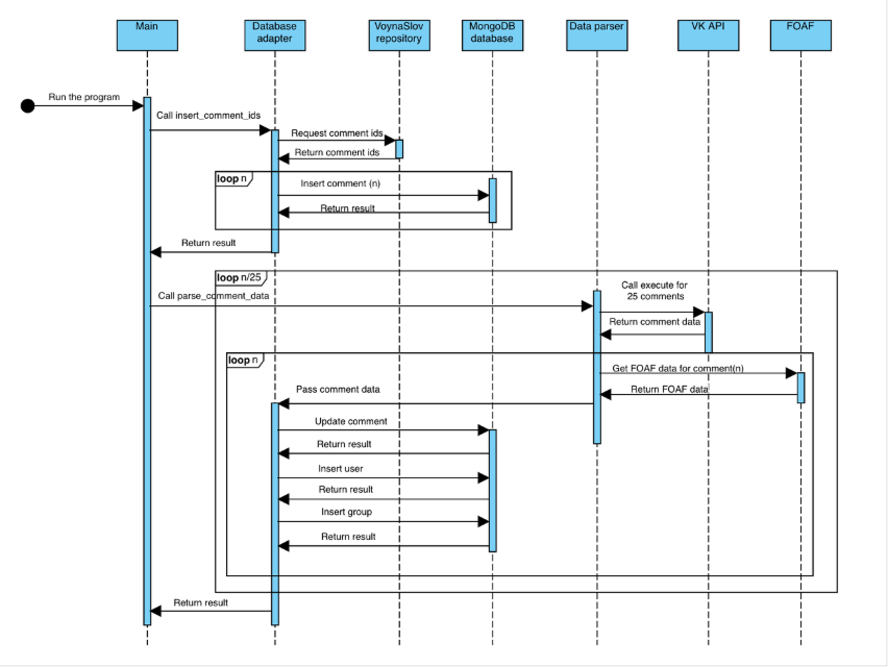
\includegraphics[width=1.0\linewidth]{Thesis/Images/sequence-diagram.pdf}
	\caption{Sequence diagram for the data collection program}
	\label{fig:sequence-data-collection}
\end{figure}

Figure \ref{fig:sequence-data-collection} presents the data collection program sequence diagram. All the steps of data processing described above are depicted in this diagram. Like this, we process all the comments from the voynaSlov repository, extract all necessary information about them from VKontakte, and save this information in the database.

\subsection{Deployment to the remote environment}
\label{sec:deployment}
The data collection program was first created and tested on the local development machine. However, as the program's database size and memory requirements grew, a need for a remote deployment environment appeared. The remote environment allows storing all the data and running the program on remote, cloud-based servers, which makes the data collection process independent of the memory and performance restrictions of the local machine.

A version control system (VCS) is necessary for this project, as it allows for easier management and distribution of the source code, including its delivery to a remote environment. Git, the most popular VCS, is used in this study. It is a free, open-source, fast and reliable system that allows branching, saving the history of modifications (commits) in the source files, and quickly switching between the branches or commits. Supplemented with Github, it also allows setting up the Continuous Integration and Delivery pipeline.

MongoDB provides a reliable cloud-based database system (MongoDB Cloud). A database with 10GB of allocated memory was created for this project. MongoDB Cloud allows the management of the database through a web interface, setting up database backups, and monitoring database metrics.

Heroku is a cloud-based platform allowing to deploy various applications. All time-consuming operations are deployed to and run on Heroku so that the data collection process does not depend on the state of the local machine. Heroku supports Docker containers, and the containers running on Heroku can access the MongoDB cloud.

In Figure \ref{fig:deployment-diagram}, you can see the deployment diagram that depicts both local and remote development environments and the relations between them and the components inside.

\begin{figure}
	\centering
	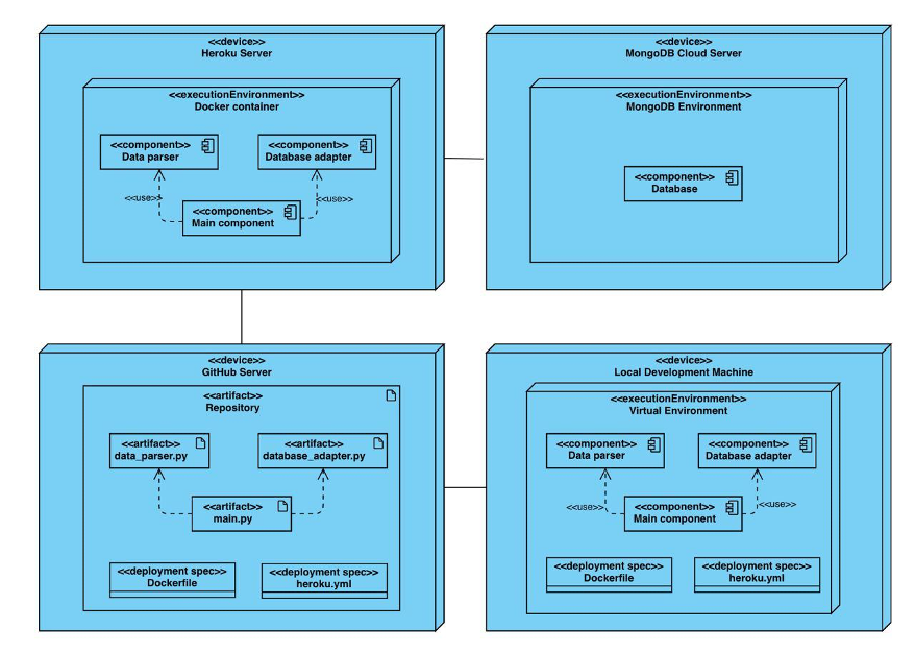
\includegraphics[width=1.0\linewidth]{Thesis/Images/deployment-diagram.pdf}
	\caption{Deployment diagram}
	\label{fig:deployment-diagram}
\end{figure}

From the local development machine, after being tested in a local virtual environment, the code is pushed to GitHub using Git. Along with the code, two configuration files are pushed: Dockerfile and Heroku.yml. The Dockerfile defines the configuration of a Docker container that should run on the Heroku server. The Heroku.yml file is a configuration file for Heroku that describes how Heroku should run the program. The code is deployed to a Heroku server from a repository on the GitHub server. A Docker container is built on this server, and all the components inside it start during the program's execution. During execution, the Database adapter component establishes a connection to the MongoDB Cloud server and makes queries, inserts and updates. The program continues to run until all comments from the initial dataset have been processed and extended information about them is stored in the database.

Running the program in a remote environment is an error-prone process. Errors can occur during the execution on the Heroku or MongoDB sides. Therefore, it is crucial to monitor the performance of the deployed program.

MongoDB Cloud and Heroku provide sufficient real-time opportunities to monitor programs and database operations execution.

Figure \ref{fig:mongodb-monitoring} shows an example of real-time monitoring in MongoDB Cloud. Using this chart, it is possible to monitor the speed and number of database queries, updates, inserts and deletes. The two most important metrics in the data collection step were ``Inserts'' and ``Updates''. During comment data parsing, we continuously update the comments collection in the database and insert documents into the ``users'' collection. Figure \ref{fig:mongodb-monitoring} shows a typical chart for unparalleled execution of these operations.

\begin{figure}
	\centering
	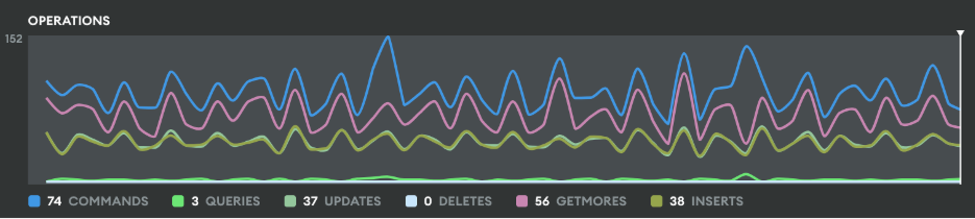
\includegraphics[width=0.7\linewidth]{Thesis/Images/database-load.pdf}
	\caption{Real-time monitoring in MongoDB Cloud}
	\label{fig:mongodb-monitoring}
\end{figure}

As seen in Figure \ref{fig:mongodb-monitoring}, the speed of database updates and inserts fluctuated around 40 per second. However, with parallelisation into three separate processes (one running locally and two running on a Heroku server) with different API tokens to avoid VKontakte restrictions, it was possible to increase the speed of both updates and inserts to 120 operations per second.

Heroku logs present another opportunity to monitor the functioning of the program online. After a deployment, Heroku starts a ``dyno'' process in several seconds. This process can crash down but will be automatically restarted by Heroku. An example of such behaviour can be seen in Figure \ref{fig:logs-monitoring}.

\begin{figure}
	\centering
	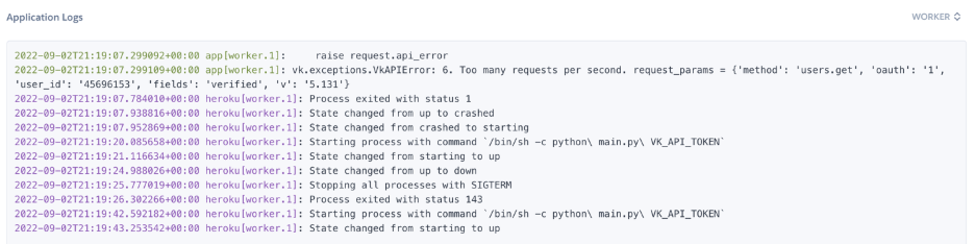
\includegraphics[width=0.7\linewidth]{Thesis/Images/application-logs.pdf}
	\caption{Logs monitoring in Heroku}
	\label{fig:logs-monitoring}
\end{figure}

It is also noticeable that Heroku logs all the errors that occur during the execution of a program, which helps debug later.

\subsection{Resulting dataset analysis}
The resulting dataset contains data about:
\begin{itemize}
    \item 5 599 287 comments;
    \item 967 groups;
    \item 283 506 users.
\end{itemize}

About 5 000 comments were not parsed from VKontakte because they had already been deleted from the platform by the time of data collection. Some users were also deleted or banned from the platform, but VKontakte stores data about them, so it was successfully parsed and stored in the database. There are 12 963 such users in the dataset. We keep all the data returned in the VK API response and some FOAF attributes for each user. There are 14 fields for each comment and 21 for each user in the database. These fields will become features for the bot detection models.

In order to successfully build bot detection models, it is necessary to conduct an exploratory analysis of the data collected. Taking a look at the dataset statistics allows us to gain insights into the data and make better use of the dataset for the model development, taking the dataset specifics into account. The exploratory data analysis was conducted on two document collections (``users'' and ``comments''). The charts below are created with MongoDB Charts\footnote{https://www.mongodb.com/products/charts}, which allows building dashboards from data stored in a Mongo database.

The ``users'' collection contains documents concerning 283 506 VKontakte users. Each of these users has a particular status at the moment of data collection. Firstly, we explore the user statuses in the database. The distribution of users by user status is shown in Figure \ref{fig:users-by-status}.

\begin{figure}
	\centering
	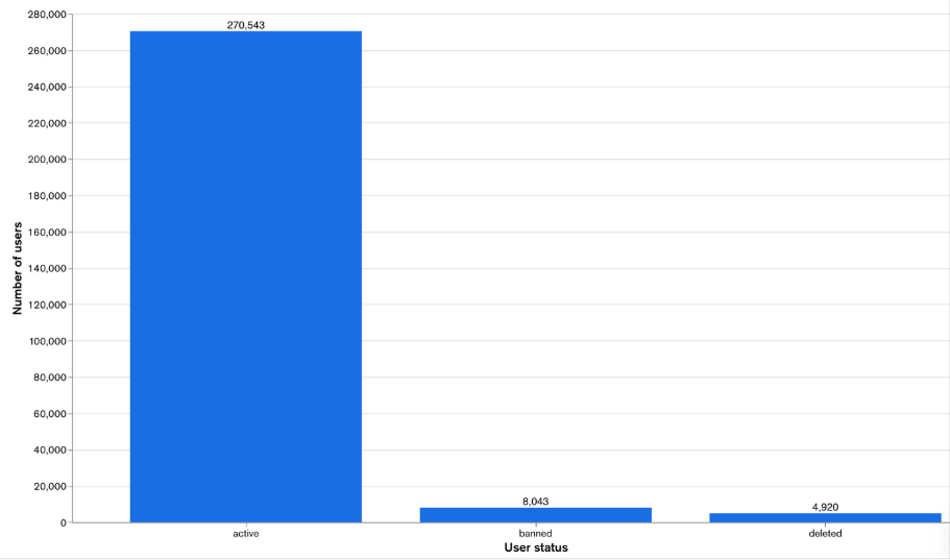
\includegraphics[width=1.0\linewidth]{Thesis/Images/users-by-status.pdf}
	\caption{Distribution of users by user status}
	\label{fig:users-by-status}
\end{figure}

It can be observed that most users (95,5\%) have an ``active'' status. Another 2,8\% and 1,7\% have a status of ``banned'' or ``deleted'', respectively. The ``banned'' status indicates that a particular user has been blocked by the VKontakte moderators. The reasons for such a block can be spamming, other fraudulent behaviour, or breaking the rules of the platform in any way. The ``deleted'' status indicates that a user deleted their account. The fact that most of the users are active on the platform is helpful for the current research, as the extended set of features from VKontakte can only be collected for active users. The data about any banned or deleted user is limited to a few fields, on which it would be hard to build a bot detection model.

Aside from the user statuses, it is also useful to explore the account creation dates of the users. We hypothesise that if there was a significant increase in the number of recently registered users, it could indicate a high number of new bots appearing on the platform. Figure \ref{fig:users-by-year} displays the distribution of users by year of account creation.

\begin{figure}
	\centering
	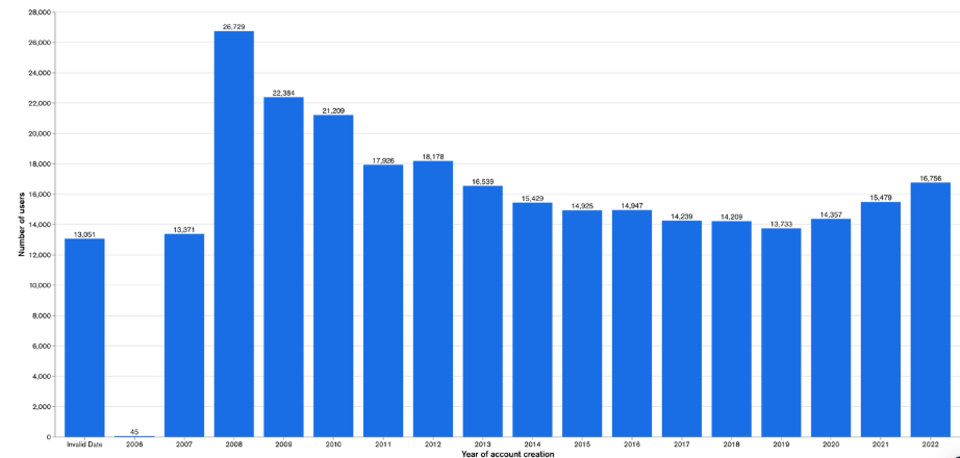
\includegraphics[width=1.0\linewidth]{Thesis/Images/accounts-by-year.pdf}
	\caption{Distribution of users by year of their account creation}
	\label{fig:users-by-year}
\end{figure}

In Figure \ref{fig:users-by-year}, an interesting pattern is observed. Since its foundation in 2006, VKontakte has attracted thousands of users each year. The peak of popularity for new users is the year 2008. During this year, 9,4\% of the users in our dataset have signed up for VKontakte. Then, the number of new registrations tends to decline. However, starting from 2019, the numbers show a positive trend. In 2022, more than 16 000 users from our dataset have registered in VKontakte. Since we only collected the data about comments left until May 2022, and 2022 is not over yet, we can suppose that by the end of this year the number of new registrations will at least double and overcome the previous record set in 2008. Therefore, a significant peak in registrations is observed during the last year. Although it is not a clear indication of a new wave of bot accounts, it can be an indirect sign of such a trend. March was the most popular month for new registrations since the beginning of 2022. In March, the number of new users that entered our dataset grew three times higher than the February level. This is shown in Figure \ref{fig:users-by-month}.

\begin{figure}
	\centering
	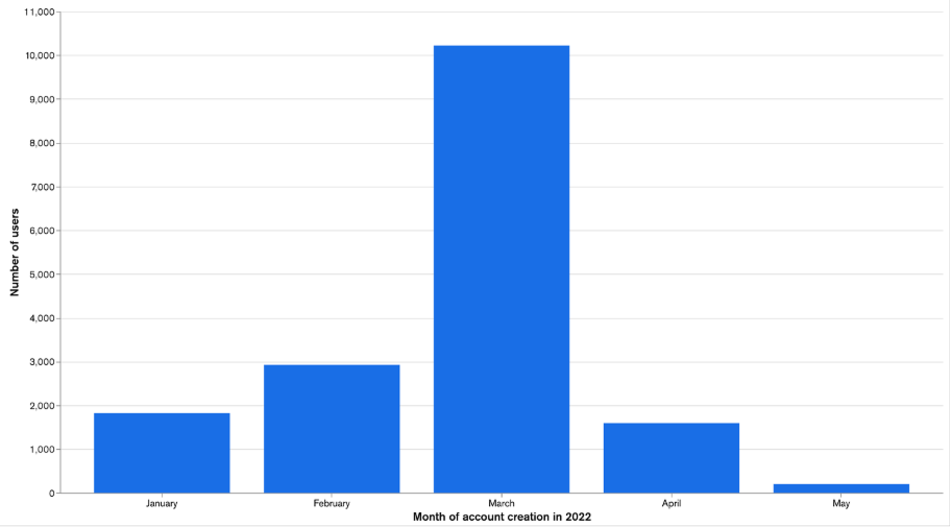
\includegraphics[width=1.0\linewidth]{Thesis/Images/accounts-by-month.pdf}
	\caption{Distribution of users by month of their account creation in 2022}
	\label{fig:users-by-month}
\end{figure}

Further, it could be helpful to explore the commenting behaviour of users in the dataset. Calculating the user activity throughout the dataset, we create a comment\_rate field in each user database entry. The distribution of the values in this field is shown in Figure \ref{fig:comments-per-user}.

\begin{figure}
	\centering
	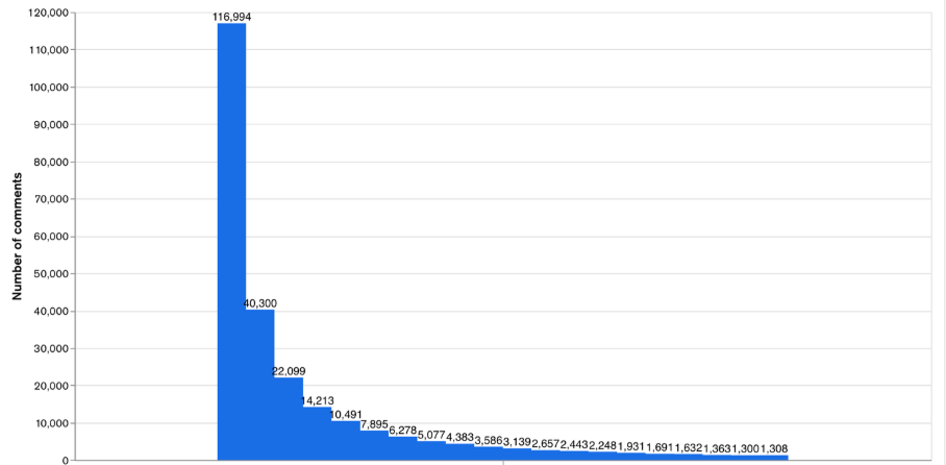
\includegraphics[width=1.0\linewidth]{Thesis/Images/comments-per-user.pdf}
	\caption{Number of comments per user}
	\label{fig:comments-per-user}
\end{figure}

In Figure  \ref{fig:comments-per-user}, a threshold of 20 comments is applied in order to make the chart more comprehensive. All the numbers higher than 20 comments are not displayed. About 41,2\% of the users only left one comment in the dataset. After the peak value at 1 comment per user, the distribution follows a declining exponent. Very few users left more than 8 comments in the dataset. This chart includes data about 251 028 users who left from 1 to 20 comments, with the remaining 32 478 users leaving more than 20 comments in the database. This behavioural peculiarity may be important for building the bot detection model.

As a conclusion regarding the ``users'' collection, most of the users in the dataset are active, and only 4,5\% of the users are banned or deleted. Moreover, we explored when the user accounts were created. There has been a slow but steady rise in the number of accounts created since 2019. The data also shows a peak in new user registrations in March 2022, which possibly can be indicative of the appearance of new bots on VKontakte. Finally, we took a look at the behavioural activity and found out that most of the users in our dataset left only one comment. Interestingly enough, some users post thousands of comments. For example, the most active user has 5 836 comments in the dataset and displays an active pro-Russian position. The second most active user has left 4 925 comments and his attitude is completely opposite (pro-Ukrainian). However, these users are rare exceptions from the overall trend with most users leaving from one to three comments.

At this stage of the analysis, it is impossible to make solid conclusions and understand who of the users is a bot and who is a real human. However, the data exploration step provides insight into the collected dataset and allows us to identify common patterns between users and detect outliers.

The ``comments'' collection contains 5 599 287 documents. Firstly, the number of valid comments is checked. About 20\% of comments in this collection are marked as invalid. This means these comments were deleted, and no data is available anymore. Several reasons can cause such a high number of invalid comments: for instance, the newly introduced Russian laws that prohibit the ``discrediting of the Russian army'' and censor social networks. Some users might have been afraid of being prosecuted for their comments and deleted them. Another reason could be the VKontakte moderator’s fight against bots and the deletion of spammy comments.

The distribution of comments by month in the year 2022 is shown in Figure \ref{fig:comments-by-month}.

\begin{figure}
	\centering
	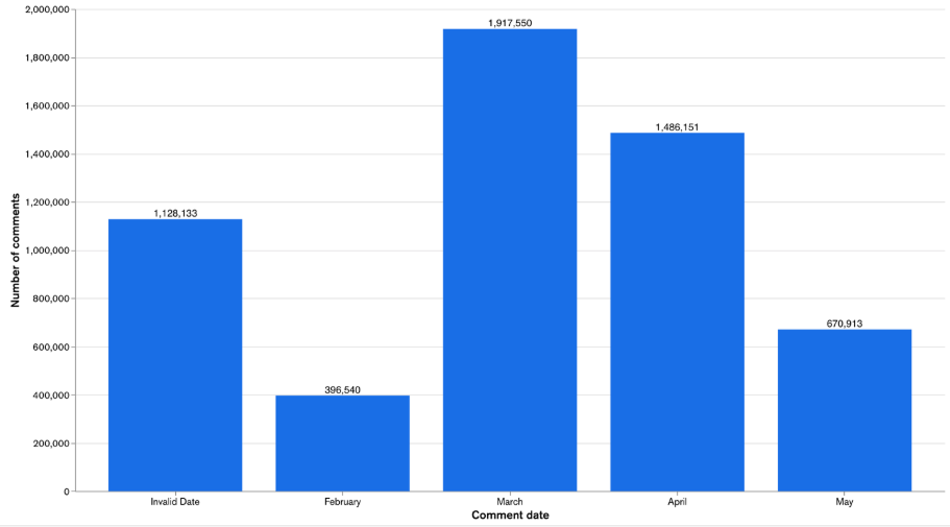
\includegraphics[width=1.0\linewidth]{Thesis/Images/comments-by-month.pdf}
	\caption{Distribution of comments by month }
	\label{fig:comments-by-month}
\end{figure}

A visible spike is observed in March with over 1 900 000 comments during this month. April’s numbers follow but are slightly lower. In May, the number of comments decreased significantly. The leftmost column marked as ``Invalid date'' represents invalid comments for which the data could not be parsed from VKontakte. It appears that VKontakte users have been talking a lot about the escalation of the Russian-Ukrainian conflict right after this escalation happened, and in March they were concerned about these events and ready for discussions in the comments. However, in May the commenting rate significantly decreased. Potentially, the users could have lost interest in the ongoing conflict, which could explain this decline.

Next, we are taking a look at the distribution of comments and posts over social media. Figure \ref{fig:posts-comments-by-media} displays this distribution in a column chart where the number of posts is marked in green colour, while the number of comments is plotted in blue. The short names of social media accounts are displayed on the X axis.

\begin{figure}
	\centering
	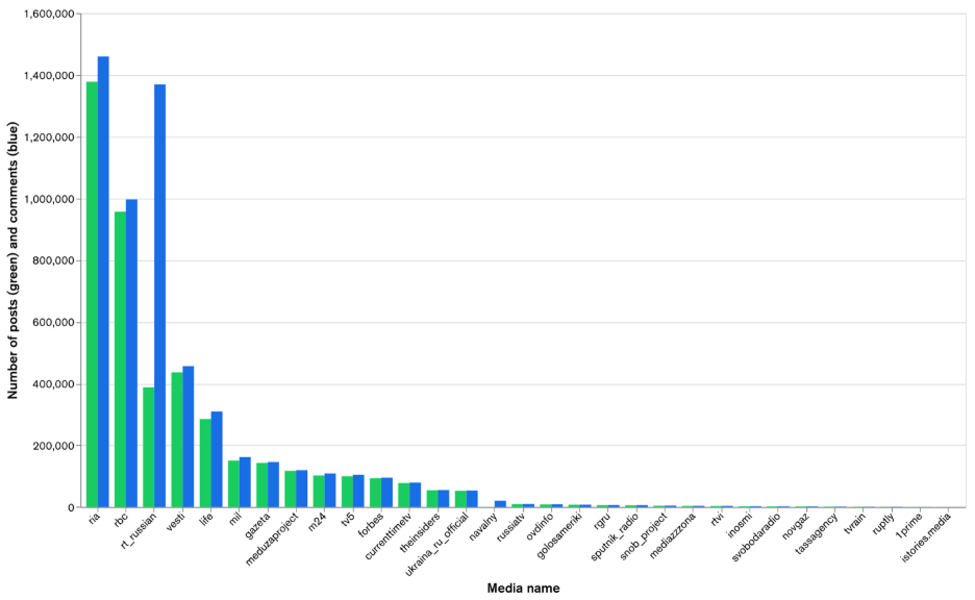
\includegraphics[width=1.0\linewidth]{Thesis/Images/comments-by-media.pdf}
	\caption{Distribution of posts (green) and comments (blue) by social media}
	\label{fig:posts-comments-by-media}
\end{figure}

The most popular social media both by the number of posts and comments is RIA. It is a state-affiliated social media, as well as RBC, RT Russian, Vesti, Life, MIL, and Gazeta, that occupy the first 6 places by the number of comments and posts. The first independent media in this list (Meduza) takes only 8th place. Overall, there is much more state-affiliated media content in the collected dataset than the content from independent media. For example, the dataset contains about 5,2 million comments on posts created by state-affiliated media and only 400 thousand comments on posts by independent media. The comment/post ratio is nearly the same (around 1,05:1) for all social media, whether state-affiliated or independent. However, RT Russian presents an exception to this rule. On average, there are 3,5 comments under each post on this social media. This anomaly is promising for further analysis and can potentially indicate the presence of bots on this social media.

\section{Building the bot detection models}
\subsection{Absence of ground truth}
Regardless of the chosen method of bot detection, the biggest challenge of this study is the absence of ground truth on which of the users is a bot. Different studies solve this problem in different ways, however, none of them is perfect. Therefore, any training of the model and evaluation of its performance is rough, approximate, and should be critically taken into account.

In most existing works where an unsupervised approach is applied, the results are evaluated and verified with the usage of existing tools such as Botometer that are believed to provide exact estimates for such models. However, Botometer does not work with VKontakte data. Moreover, Botometer is claimed by some researchers as an unreliable bot detection tool because of a high number of false positives \cite{Gallwitz2022}. Therefore, it is not possible to copy the evaluation strategy from existing work. In \cite{Alymov2016}, the authors provide three alternatives to Botometer that can be used with VKontakte data, namely, Akismet, Vkontakte Antispam and ``Research weight of RuNet''. The first tool requires comment features that VKontakte does not provide, such as IP address. The second tool has not been updated for three years and is not working now. The third tool has also been removed from the Internet.

Another tool similar to Botometer exists for VKontakte. It is called GosVon and provides a database with VKontakte users labelled as bots\footnote{https://gosvon.net/}. However, the method on which the GosVon is based is unclear and not described on their website. There is no information regarding the performance and accuracy of this method. Moreover, the project aims to expose only pro-Russian bots, and it doesn’t take into account any other types of bots. Thus, the labels from this dataset are to be treated carefully and cannot be guaranteed to provide the ground truth.

Some of the user profiles on VKontakte contain a ``deactivated'' feature that can take the value of either ``deleted'' or ``banned''. The banned users should most likely be bots. However, taking the banned users as a gold label for social bots is not the perfect approach to the model evaluation. The reasons for that are:
\begin{itemize}
    \item VKontakte moderators may ban users for different reasons than being a bot. For instance, real users spreading inappropriate content may be blocked.
    \item VKontakte moderators might miss some recently created bot accounts. Probably, they do not have enough time to check new bot accounts.
    \item VKontakte is a company with tight relations with the Russian government. Gazprom, a state-owned Russian gas company, has been the biggest shareholder of this social network since 2021\cite{vkgazprom}. Therefore, objectivity and transparency of VKontakte's moderators' work cannot be guaranteed.
\end{itemize}

Taking a look at the problem from a different perspective, we aim to understand which users are guaranteed to be real ones, not bots. The thesis author is registered on VKontakte since 2009 and has been an active user for more than 10 years. The thesis author is sure that all of her 204 friends on VKontakte are real people. Moreover, likely, the friends of the author's friends are also real people. Thus, if a user is a friend of the author or a friend of a friend, this user is probably not a bot.

In the collected dataset, there are only 3 author's friends and 308 friends of friends. These users can be seen as a standard of a real user with a high probability.

Another method by which it is possible to identify real users is by analysing the ``verified'' field returned from VKontakte. This field is true only for the users who have verified their identity using their official documents. Surprisingly, there are only 37 such users in our dataset of 5,6 million comments.

The two approaches above guarantee that 348 users out of 5,6 million are real humans. On its own, measuring how well the model performs on these users does not provide us with enough information to evaluate the model as a whole. However, evaluation on these users can be a part of the overall evaluation strategy.

The manual evaluation was also considered a possible evaluation method. However, this method presents several difficulties:
\begin{itemize}
    \item The size of the dataset does not allow for a manual evaluation of the whole dataset in a reasonable amount of time.
    \item The accuracy of manual evaluation can be low. In one study, human evaluators have only been able to correctly label 24\% of the bots\cite{Cresci2017a}. ``Humans can not detect sophisticated bots in most scenarios''\cite{Kolomeets}.
\end{itemize}

In some papers regarding bot detection on VKontakte, e.g. \cite{Kolomeets2021} and \cite{Kolomeets2021a}, the authors inject social bots to VKontakte and evaluate their models using these bots. While being a valid approach in other contexts, in the current research, it does not seem to be a suitable method. Injecting additional bots into VKontakte is not moral in the context of an ongoing armed conflict, can further destabilise the political situation in Russia and Ukraine and negatively influence the social landscape of the VKontakte community. Thus, we will not inject any bots spreading political propaganda in VKontakte.

As a summary of the above, the scientific community does not currently have a 100\% reliable method of obtaining the ground truth for the bot detection task that this study aims to solve. Therefore, a combination of the most reliable methods will be used to evaluate the performance of models built in the course of this research. We will consider verified users and those users who are in our friends network as real humans, and will additionally label a subset of users via crowdsourcing to gather independent opinions on whether some users from the dataset or bots or humans. This approach will allow evaluation of the model performance with some degree of certainty. 

\subsection{Labelling process}
\label{sec:labelling}
Due to the unreliability of individual judgment, we rely on several independent labels to obtain a summarized label for a small subset of users from the dataset. The labels are collected via a survey launched on the Prolific\footnote{https://www.prolific.co/} platform. As a first step, it is necessary to find suitable respondents for the study. The respondents will have to inspect VKontakte accounts, posts and comments written by users from the dataset. Therefore, there are several criteria that the respondents should satisfy: they should have a VKontakte account and be fluent in both Russian and Ukrainian, since these two languages are the most popular in the dataset. Moreover, we filter the respondents by education level (at least Bachelor level) and approval rate (at least 95\%). There were 250 such respondents on Prolific.

Next, we choose samples of users from the database to run the labelling process on. The first sample is entirely random and consists of 100 users. The randomness of the sample is ensured by using the \$sample\footnote{https://www.mongodb.com/docs/manual/reference/operator/aggregation/sample/} aggregation stage in MongoDB. It is designated to be used to evaluate the Friendship relations method, described later in \ref{sec:friendship-relations}. The second and third samples consisted of 20 users each and are related to each of the methods used to build the bot detection model (URL sharing and Hashtag sequences). These methods are described in detail in further sections \ref{sec:image-url-sharing} and \ref{sec:hashtag-sequences}. The IDs of users to label were selected manually for the second and third sample from suspicious and normal clusters identified by the URL sharing and Hashtag sequences methods. 

Labelling each user requires quite a thorough inspection of their profile and comments that they have written on VKontakte. We estimated that it would take each respondent up to five minutes to label each user. Therefore, the number of users to label per respondent was limited to 10 so as to take them less than an hour to complete. For each user from the samples, we aimed to collect at least three labels to obtain a more objective summarised label.

Launching the survey on Prolific required building a separate web interface to enable user labelling. This web interface is connected to the database via the web backend. To each respondent, this interface offers to firstly enter their Prolific ID in order to allow respondent identification later on. Next, the respondent is presented with a short description of the survey goals and the respondent's tasks. This description also contains the definitions of a social bot and real human account, so that respondents can better understand the context of the survey. The interface subsequently presents 10 users from the samples to the respondent and offers two buttons: ``BOT'' and ``HUMAN''. According to the personal judgement, after inspecting the user's VKontakte account and comments, the respondent decides which button to press. The user flow of the labelling process is shown in Figure \ref{fig:labelling-user-flow}.

\begin{figure}
	\centering
	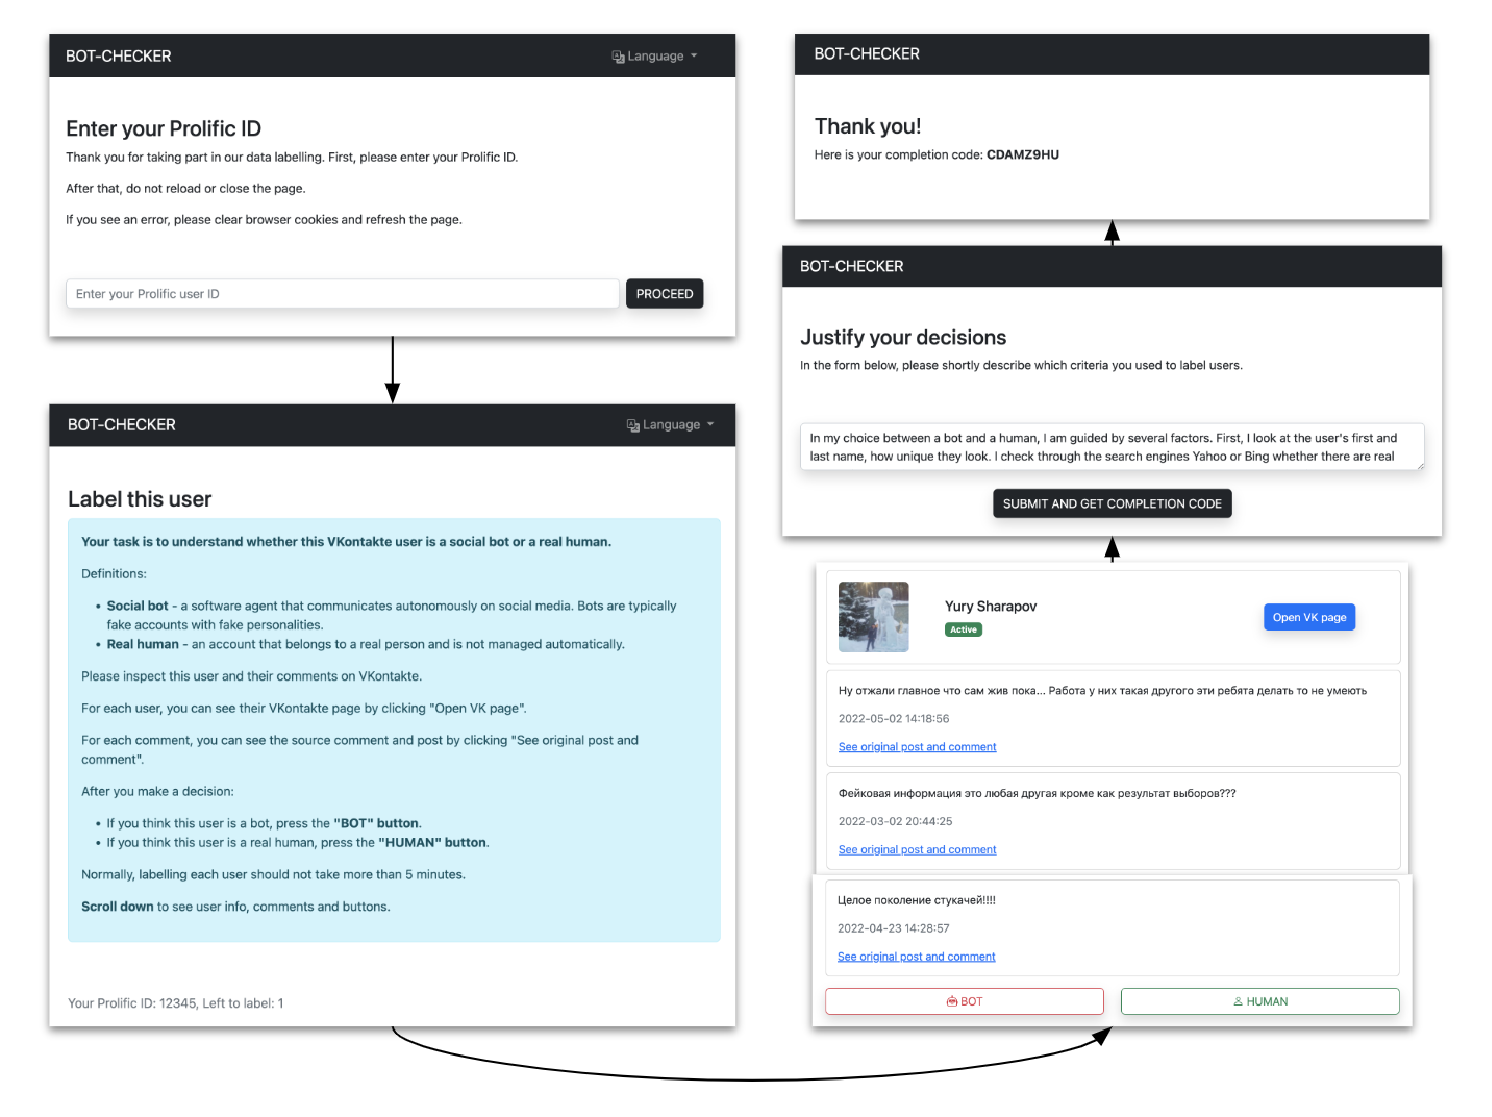
\includegraphics[width=1.0\linewidth]{Thesis/Images/labelling-web-interface.pdf}
	\caption{The labelling interface user flow}
	\label{fig:labelling-user-flow}
\end{figure}

In the end, respondents are asked to justify their labelling choices in a free-form text entry. By reading these comments, we can gain valuable insights into the features that respondents take into account when labelling users. From the respondents' free text responses, it was also obvious that one respondent was too subjective while labelling users. This person claimed that any VKontakte user with anti-Russian position was spreading fake news and propaganda by default and had to be labelled as bot. However, this user's labels did not skew the labelling results due to the presence of at least two other opinions for each user from the samples. 

The characteristics that respondents used to label users are depicted in Figure \ref{fig:labelling-principles}. As we can see, most respondents paid attention to the photos, and especially to avatar pictures, of the users they checked. The following popular characteristic was the meaning of comments and the suitability of comments to the post. Respondents also paid attention to the posts and reposts of a user and to the friends list. Very few respondents checked for the features that might, according to the methods applied in this study, be indicative of bots. For example, only four respondents took into account the URLs or hashtags that VKontakte users share in their comments. 

\begin{figure}
	\centering
	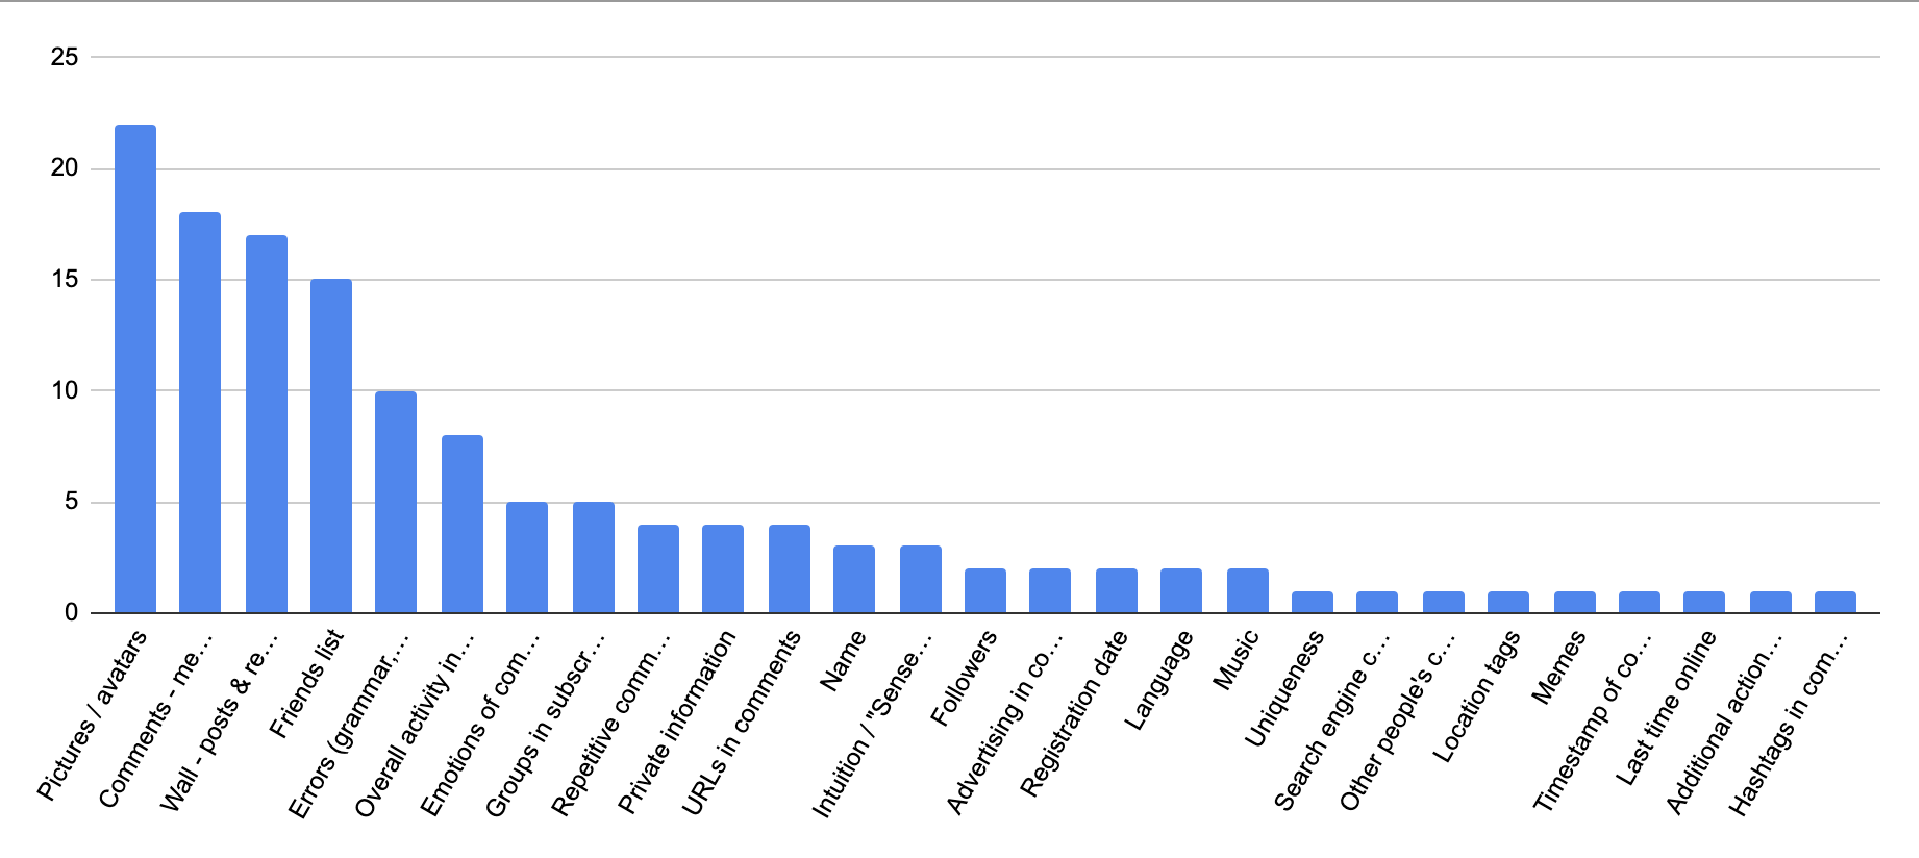
\includegraphics[width=1.0\linewidth]{Thesis/Images/labelling-principles.pdf}
	\caption{Characteristics that influenced labelling outcomes}
	\label{fig:labelling-principles}
\end{figure}

As a result of the labelling process, we obtained labels for 139 users from the dataset. One hundred users belonged to the first random sample. 20 and 20 users belonged to the second (URL sharing) and third (hashtag sequences) samples, respectively. There was an overlap in the case of one user who belonged to the second and third samples simultaneously. When calculating the resulting label, we adhered to the majority principle (e.g. if there were 2 ``Bot'' labels and 1 ``Human'' label, the resulting label was ``Bot''). In case of a tie (13 cases), we labelled the user ourselves to obtain another opinion and calculate the resulting label.  Out of 139 users labelled, 33 users were labelled as bots and 106 as humans. Therefore, the respondents considered 23\% of the sample users to be bots. This percentage is higher than the number from previous research on VKontakte bots that claimed that 17\% of users on this platform are bots\cite{vkBotPercentage}. 

The resulting labels that we obtained as a result of the Prolific survey, along with other account features, will be used as the gold standard to measure the performance of the model and draw conclusions about its efficiency.

\subsection{Initial choice of method}
The method selection phase consisted of the following steps:
\begin{enumerate}
    \item Refining the search query. In order to avoid irrelevant methods, the search query should be as precise as possible. After several iterations of search query refinement, the most relevant results were obtained under the following query:
           unsupervised AND method AND ``social network''
           AND ``bot detection'' AND(politics OR propaganda)
           -survey
    \item Refining the time range. Since group-based approaches started gaining popularity only in 2018\cite{Cresci2020}, the time range was limited to 2018-2022.
    \item Downloading the data. To do this, the scientific software Publish or Perish\footnote{https://publish-or-perish.en.softonic.com/} was used. In total, 130 papers that matched the search query and the time range were downloaded.
    \item Filtering out the articles that were never cited by any scientists. Since a higher citation score can indicate a more trustworthy paper, all the papers with a citation score of 0 were excluded. After that, only 81 articles remained.
    \item Manually analysing the titles one by one. Titles summarize the papers and can give a general impression of the work described in each paper. During the manual selection, 53 papers were identified as potentially relevant to this thesis.
    \item Preferably, the methods used in this research should have already been applied in the context of either politics in general or Russian politics in particular. Therefore, each article was identified as politics-related or not. In the politics-related ones, an additional classification for Russia-related and other papers was made. 14 of the papers were marked as politics-related, three of them as Russia-related.
    \item Abstract analysis. The abstracts of the 14 papers were scrutinized to understand if these papers present methods applicable for the current research. Only 9 papers were left after this examination.
    \item Paper analysis. The methods presented in the remaining 9 studies are further examined, and the following characteristics are identified (Table \ref{tab:bot-detection-methods}
    \begin{itemize}
        \item Approximate computational complexity and time. As the current research makes use of a large quantity of data, this characteristic is crucial for success. Lower computational complexity and time will allow running the method on all the data collected.
        \item Performance. This can be measured by F-score or ROC AUC in various papers. Bot detection quality is crucial to building an efficient and reliable bot detection model.
        \item Features and data used, and applicability to VKontakte. The method should be adaptable to VKontakte data specifics, such as the user or comment features, and should not depend on Twitter-specific features.
        \item Availability of the code. If the authors of a method provide open source code to support their work, it becomes easy to reproduce their research.
    \end{itemize}
\end{enumerate}

\begin{table}[]
\caption{Methods selected in the first iteration of model selection process}
\label{tab:bot-detection-methods}
\begin{tabular}{llllll} \toprule
\textbf{\#} & \textbf{Type} & \textbf{Performance}                                                             & \textbf{Works for VK} & \textbf{Open code} & \textbf{Source} \\ \midrule
1           & Supervised          & \begin{tabular}[c]{@{}l@{}}Precision=78.5\%\\ ROC AUC=0,99\end{tabular}          & Yes                       & No                      & \cite{Im2020}        \\
2           & Supervised          & \begin{tabular}[c]{@{}l@{}}Accuracy=93,2-96,2\%\\ ROC AUC=0,98-0.99\end{tabular} & Yes                       & Yes                     & \cite{PastorGalindo2020}       \\
3           & Supervised          & ROC AUC=0,79-0,89                                                                & Yes                       & No                      & \cite{Alsmadi2020}        \\
4           & Supervised          & Accuracy=83\%                                                                    & Yes                       & Yes                     & \cite{Rossi2019}       \\
5           & Supervised          & Accuracy=83\%                                                                    & Yes                       & No                      & \cite{Rossi2020}      \\
6           & Unsupervised        & No data                                                                          & Yes                       & No                      & \cite{Nizzoli2021}        \\
7           & Unsupervised        & Accuracy=86\%                                                                    & Yes                       & Yes                     & \cite{Hagen2022}        \\
8           & Unsupervised        & No data                                                                          & Yes                       & No                      & \cite{Hanouna2019}        \\
9           & Unsupervised        & Various                                                 & Yes                       & No                      & \cite{Riofrio2018}  \\ \bottomrule
\end{tabular}

\end{table}
 
Judging by the Table \ref{tab:bot-detection-methods}, only 4 methods out of 9 are suitable for the current research due to their unsupervised method type. Out of these, only method 4 provides an estimate for accuracy. Moreover, method 7 provides the code to reproduce it. Therefore, for the current research, the seventh method is initially chosen.

The method was applied to the 2016 US elections data from Twitter. It consists of five consequent steps:

\begin{enumerate}
    \item Employing a community detection algorithm to define the network structure and identify unique communities based on retweet relations.
    \item Usage of a series of bot detection algorithms to identify the likelihood of each node in the network being a social bot.
    \item Calculation of several commonly used centrality measures to identify influential actors in each of the detected communities.
    \item Sentiment analysis to better understand the tone and content of the information communicated in the network as a whole as well as in each individual community.
    \item Content analysis to describe the categories of user profiles in order to identify the types of actors who were most influential in the discussion network.
\end{enumerate}

All of these steps can be applied to our dataset, except for the second. In the
original paper, the authors use Botometer and tweetbotornot. There are no alternatives for these tools that could be used with VKontakte data. Therefore, this step is omitted.
In step 1, the authors build a network of users based on the retweeting behaviour. Since there are no retweets on VKontakte, a different measure for building the network should be chosen. A graph of users can be built based on either of these aspects:
\begin{itemize}
    \item Friends graph (as stated in \cite{Kolomeets2021}, friends structure can be indicative of bots.
    \item Users similarity (building a weighted graph with user similarity as in \cite{Fazil2020}).
\end{itemize}

Since building the graph based on users' similarity would involve calculating the similarity metric more than 80 milliard times (283 506 squared), which is very computationally heavy and would take a significant number of days, a decision was made to base the graph on the friendship connections between users.

\subsection{Friendship relations}
\label{sec:friendship-relations}
In the original paper \cite{Hagen2022}, the user graph was based on retweet behaviour. Since VKontakte does not have a tweeting/retweeting feature, an alternative should be found. As stated in \cite{Kolomeets2021}, it is possible to identify bots by friend structure. Therefore, a graph can be built based on the friends' network. For each of the 283 506 users in the database, the additional field was parsed from VK API, containing the list of their friends. Then, for each user, this list is matched against the database users, and an intersection between the friends' list and the ``users'' collection is found. A graph depicting these friendship relations consists of nodes (represented by user IDs) and edges (representing the friendship relation between users).

To cluster the model, the Louvain clustering algorithm is used\cite{louvainalg}. In the original paper\cite{Hagen2022}, this algorithm is chosen because of the ``easy implementation and high-quality results''.  In the end, the algorithm finds clusters with maximal modularity. Louvain clustering is widely used for community detection on social networks (for example, in \cite{louvaindynclust}, \cite{de2011generalized}, \cite{sanchez2016twitter}).

For this study, the implementation of the Louvain algorithm from the popular and widely used python-louvain library\footnote{https://github.com/taynaud/python-louvain} was chosen. This library takes advantage of NetworkX\footnote{https://networkx.org/}, a Python package for graph management.

The data about friends could only be fetched for 167 276 users. The other users have either hidden their friends lists from the public, or were deleted or banned. Therefore, only 167 thousand users have been used to form clusters. The user graph itself was formed by 73 253 nodes, each node corresponding to a user. These are the users that are connected to at least one other user in the graph. The Louvain clustering produced 5 478 unique clusters that were saved to a MongoDB collection.

After clusterisation, the Gephi software was used to create a visual representation of the clustered graph. Like in the original paper\cite{Hagen2022}, we used the ForceAtlas 2 layout for the graph visualisation because it produced the best visually understandable cluster layout.


\subsection{Subsequent choice of method}
Building graph based on friendship relations only produces large clusters and might not be accurate. So in order to find a suitable method for more granular and precise bot detection, we now pay attention to the methods that were previously found during initial method selection but were filtered out some stage of the analysis. Instead of taking into account features like open source code availability and applicability to VKontakte data, we rely more on qualitative analysis of titles, abstracts and full texts. 

Out of 96 papers, we select 18 as the most suitable judging by the title and abstract. Having read through these 18 papers, we find one that presents a group-based unsupervised method applied to 5 different case studies with modifications. This is a study named ``Uncovering Coordinated Networks on Social Media'' \cite{pacheco2020uncovering}. The paper provides a core framework, on the basis of which five different models are built and applied to various datasets, including data from Hong Kong protests, US elections and other major political events. The framework is general and therefore versatile, allowing to hypothesise that it can be suited for the task of bot detection in VKontakte.

In the framework, several steps are proposed to detect bots:
\begin{enumerate}
    \item Behavioral trace extraction. From a dataset containing tweets, we extract some behavioural features based on which users can be united into a network. These features, or traces, might indicate suspicious coordinated behaviour.
    \item Bipartite network construction. A ``user-to-feature'' bipartite graph is constructed.
    \item Projection onto account network. The bipartite graph is projected onto a user graph, and weights are derived by some transformation from the initial bipartite network weights. 
    \item Cluster analysis. The resulting user network is analysed manually to identify ``suspicious'' and ``normal'' clusters with high potential number of bots or humans, respectively.
\end{enumerate}

To this framework, we add an additional step: comparison of the model results with the labelling results (\ref{sec:labelling}). This allows to estimate each model's performance using standard metrics, such as accuracy, precision and recall. We then compare the resulting models and make conclusions about each model's applicability to the case of bot detection on VKontakte.

The success of a bot detection model built with this framework depends on the choice of initial behavioural traces considered suspicious. In the five case studies, these traces are different:
\begin{enumerate}
    \item Account handle sharing;
    \item Image coordination;
    \item Hashtag sequences;
    \item Co-Retweets;
    \item Synchronised action.
\end{enumerate}

From these five types of traces, only Image coordination, Hashtag sequences and Synchronised action apply to our dataset. Moreover, the Synchronised action method is the least efficient and therefore not suitable for the large dataset size. Thus, in the subsequent sections, we will explore the application of Image coordination and Hashtag sequences methods to the task of this research.

\subsection{Image and URL sharing}
\label{sec:image-url-sharing}
The method used in \cite{pacheco2020uncovering} to detect coordinated communities of bots during the Hong Kong protests of 2019 utilises image similarity to construct a user graph. More specifically, it first examines tweets by various users, extracts the images from them and creates RGB histograms for each image. At first, the same method was meant to be applied to our dataset. However, we soon realised that VKontakte API does not allow obtaining raw image data by image URL. Therefore, when parsing image URLs from comments, we could not create histograms for VKontakte images. It was only possible to do so for images hosted on some external websites. However, the majority of users shared only VKontakte images. Therefore, building a complete graph with image histograms was not possible.

Instead of building a graph based on image similarity, we have built it based on URL-sharing patterns. The approach was similar to the image similarity method, except that for links, there was no need to create any histograms. They could just be compared for equality. The complete URL sharing method consisted of the following steps:
\begin{enumerate}
    \item Retrieve URLs from all comments using a regular expression;
    \item Create a bipartite graph that connects users to URLs, where edge weights are determined by how often a user shares a specific URL;
    \item Perform a projection of the bipartite network to obtain a weighted account coordination network, with weights of edges calculated using the bipartite network weights with Jaccard similarity metric;
    \item Visualise the graph with Gephi and identify ``suspicious'' and ``normal'' clusters.
\end{enumerate}


\subsection{Hashtag sequences}
\label{sec:hashtag-sequences}
The Hashtag-sequences method from \cite{pacheco2020uncovering} is also applied to the same dataset in order to build a different group-based model and compare it with the URL-sharing model. The Hashtag-sequences model is based on the same steps as the URL-sharing model. However, the main feature with which we capture account similarity is not the similarity of URL that users share, but the similarity of hashtag sequences they share in their comments. In the original study\cite{pacheco2020uncovering}, this method is applied to the case of US elections discussion on Twitter. 

\subsection{Evaluation}

To evaluate and compare the three bot detection methods, we calculate standard metrics:
\begin{itemize}
    \item Accuracy: $(TP+TN)/(TP+FN+TN+FP)$
    \item Precision: $TP/(TP+FP)$
    \item Recall: $TP/(TP+FN)$
\end{itemize}

Accuracy tells how many times the model was correct overall. Precision is how good the model is at predicting a specific category. Recall tells how many times the model detected a specific category\footnote{https://www.mage.ai/blog/definitive-guide-to-accuracy-precision-recall-for-product-developers}. The higher all three metrics, the more successful we consider a bot detection model. It is not sufficient to have just one or two of these metrics with a high value because that might mean that a model is good at predicting one class (e.g. humans) but fails at predicting the other (e.g. bots).

\subsection{Exploring influentialness}
To identify influential users in clusters, a centrality metric Degree Centrality and a clustering coefficient are calculated. To compute these values, standard NetworkX functions are used.

Degree centrality can be a measure of influentialness of an actor in the graph\cite{Hagen2022}.  The clustering coefficient ``of node A measures the extent to which the neighboring nodes of A form a densely clustered clique''\cite{Hagen2022}. Higher clustering coefficients in a network show stronger connections among actors in that community\cite{Hagen2022}. 

To estimate bots' influentialness, we calculate these two metrics for two user networks: before bot removal and after bot removal. This allows us to see how the influentialness metrics change due to bots' presence. The same "before-and-after" approach is applied to sentiment analysis.

\subsection{Comment language detection}
Since the dataset may contain content produced in various languages, including, primarily, Russian and Ukrainian, but also potentially English, it is crucial to identify the language in which each comment is written. This will help in further sentiment analysis. To detect language, a popular langdetect\footnote{https://pypi.org/project/langdetect/} Python library is used. It is a re-implementation of Google’s Java language-detection library.

Surprisingly, after the first iteration of language detection for the comments in the database, the third and fourth most popular identified languages were Macedonian and Bulgarian.

However, after a close manual examination of a sample of 1000 comments, it became clear that comments labeled as ``Macedonian'' contained of Russian text in 99\% of the cases. Examples of comments misclassified by the langdetect library are given in Figure \ref{fig:misclassified-comments}.

\begin{figure}
	\centering
	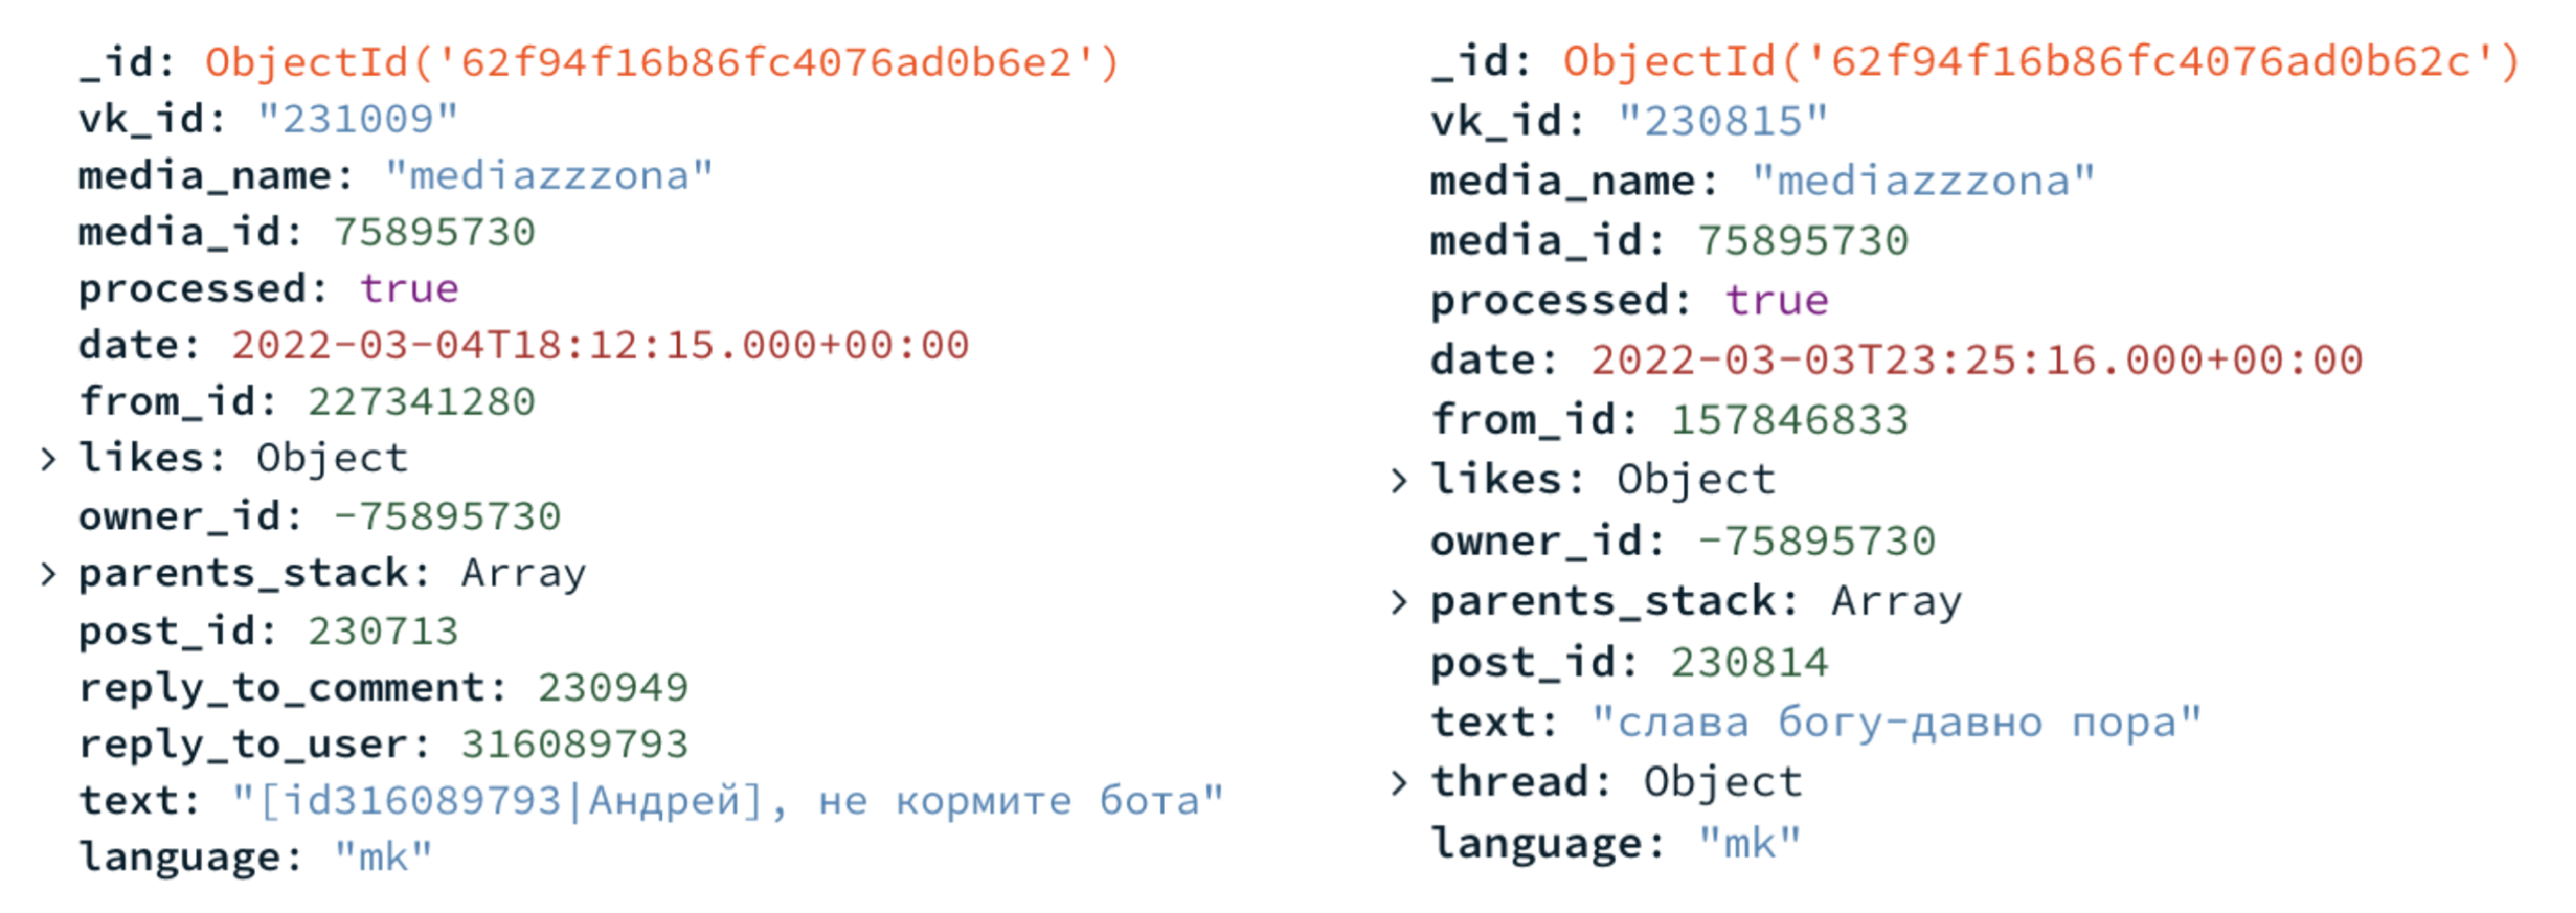
\includegraphics[width=0.8\linewidth]{Thesis/Images/misclassified-comments.pdf}
	\caption{Comments containing Russian text and misclassified as Macedonian}
	\label{fig:misclassified-comments}
\end{figure}

The same could be observed for comments identified as containing Bulgarian language. Therefore, all the comments classified with ``mk'' or ``bg'' language codes were updated to be classified as Russian text.

After that, the distribution of languages became as displayed in Figure \ref{fig:comments-by-language}.

\begin{figure}
	\centering
	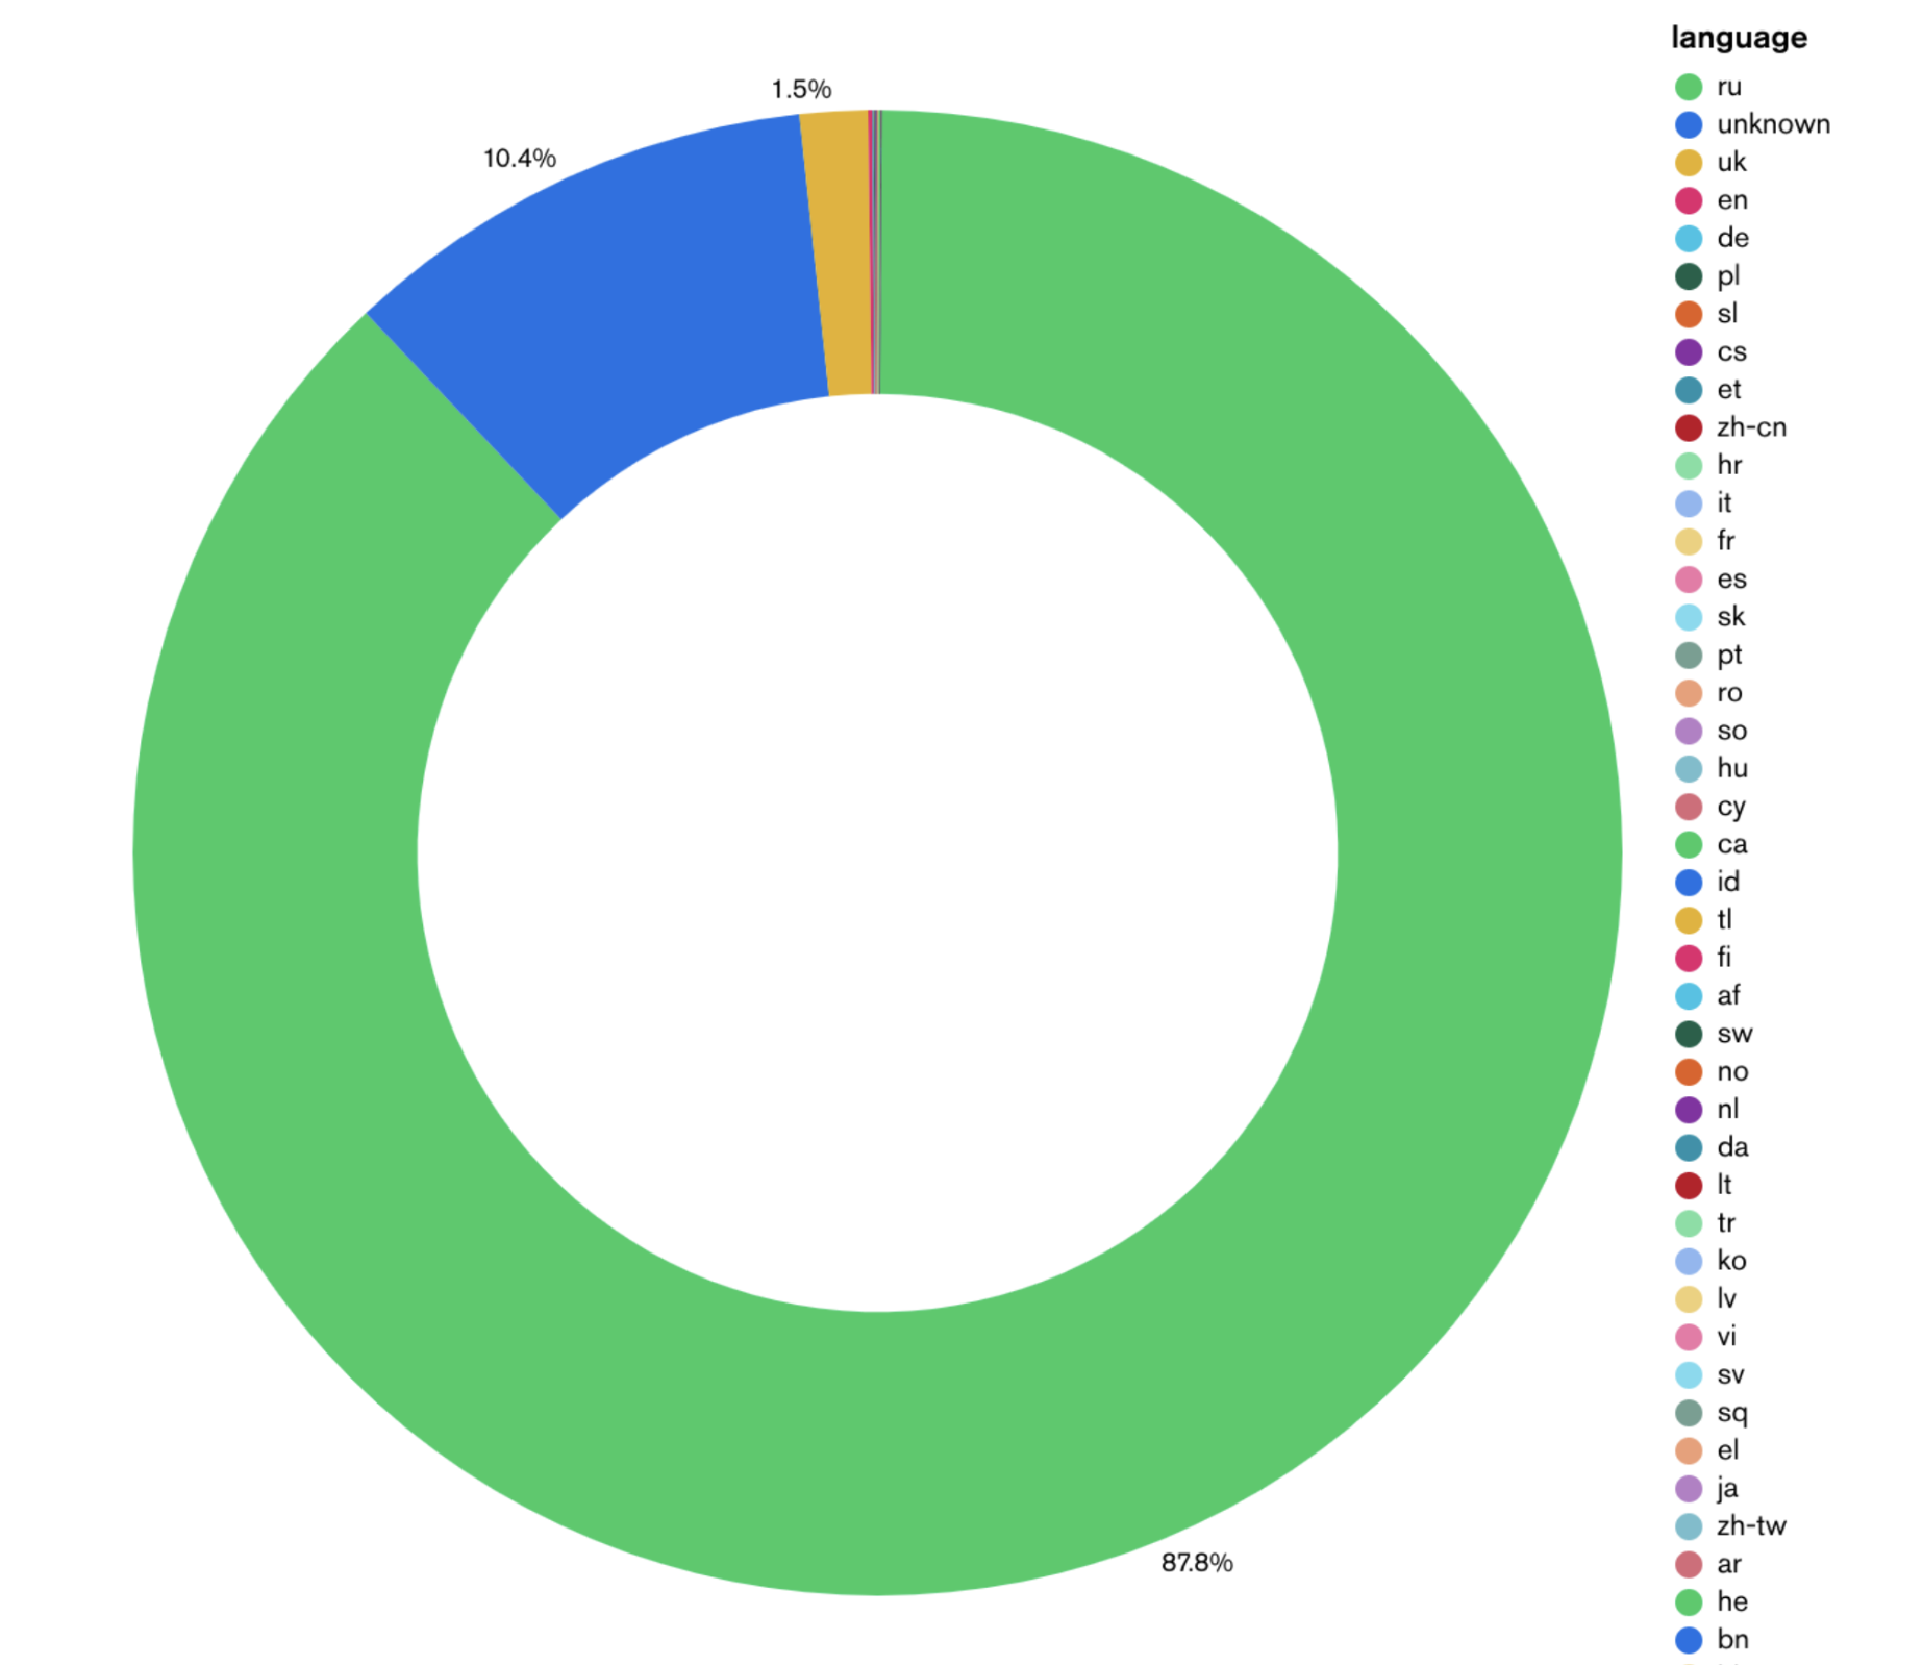
\includegraphics[width=0.8\linewidth]{Thesis/Images/comments-by-language.pdf}
	\caption{Distribution of comments by language}
	\label{fig:comments-by-language}
\end{figure}

The most popular language in the dataset is Russian with 87.8\% of comments. The second most frequent value is ``unknown'' (10.4\%). This label is used in four possible cases:
\begin{enumerate}
    \item When a comment consists of user tagging without any additional text;
    \item When a comment consists of emoji only;
    \item When a comment does not contain any text;
    \item When the langdetect library cannot detect a language for the comment.
\end{enumerate}

The Ukrainian language is the third most frequent value in our dataset with 1.5\% comments written in this language.

The rest 0.3\% of the comments were identified as written in languages other than Russian and Ukrainian. After a manual examination, we came to the conclusion that the language was identified incorrectly for most of these comments. In absolute numbers, the number of incorrectly identified comments is quite big (about 17 thousand comments), but relatively, it’s a small fraction of the dataset. Therefore, for further analysis, these comments will not be taken into account for the sake of simplicity.

As a result of the language detection step, the ``language'' attribute was defined for each valid comment in our database. The most popular languages are, as expected, Russian and Ukrainian. Russian language dominates over Ukrainian in our database. This can be explained by the fact that most of VKontakte users (82.38\% come from Russia, while only 3.22\% come from Ukraine\cite{vkGeography}.

\subsection{Exploring comment sentiment}

Conducting sentiment analysis on comments written in English or Russian is quite a widespread task that has established popular solutions. In the original paper where the authors analysed English content, they used the SentiStregnth model. It currently supports 16 languages. However, Ukrainian is not one of them. Moreover, the Ukrainian sentiment analysis research does not offer widely adopted methods and models. Even in the most recent articles dedicated to the Russian-Ukrainian conflict of 2022, sentiment analysis is conducted on texts written in English (e.g. \cite{caprolu2022characterizing}). Thus, conducting direct sentiment analysis for Ukrainian texts presents an unsolved task and cannot be applied to this study. Instead, as Russian and Ukrainian share a common Slavic root, we hypothesise that translating Ukrainian comments to Russian will not lead to a significant loss in meaning. After this translation, it will be possible to conduct sentiment analysis on the translated text.

Just as in the original paper\cite{Hagen2022}, we use the SentiStregnth model. The Python version of this library\footnote{https://github.com/zhunhung/Python-SentiStrength} allows integrating the sentiment analysis into our data processing pipeline. SentiStrength outputs scores from 1 (not positive) to 5 (extremely positive) for the ``positivity'' of a piece of text and scores from -1 (not negative) to -5 (extremely negative) for the ``negativity'' of text. Both scores were calculated and saved to the database for all the comments written in Russian and Ukrainian language.

\begin{figure}
	\centering
	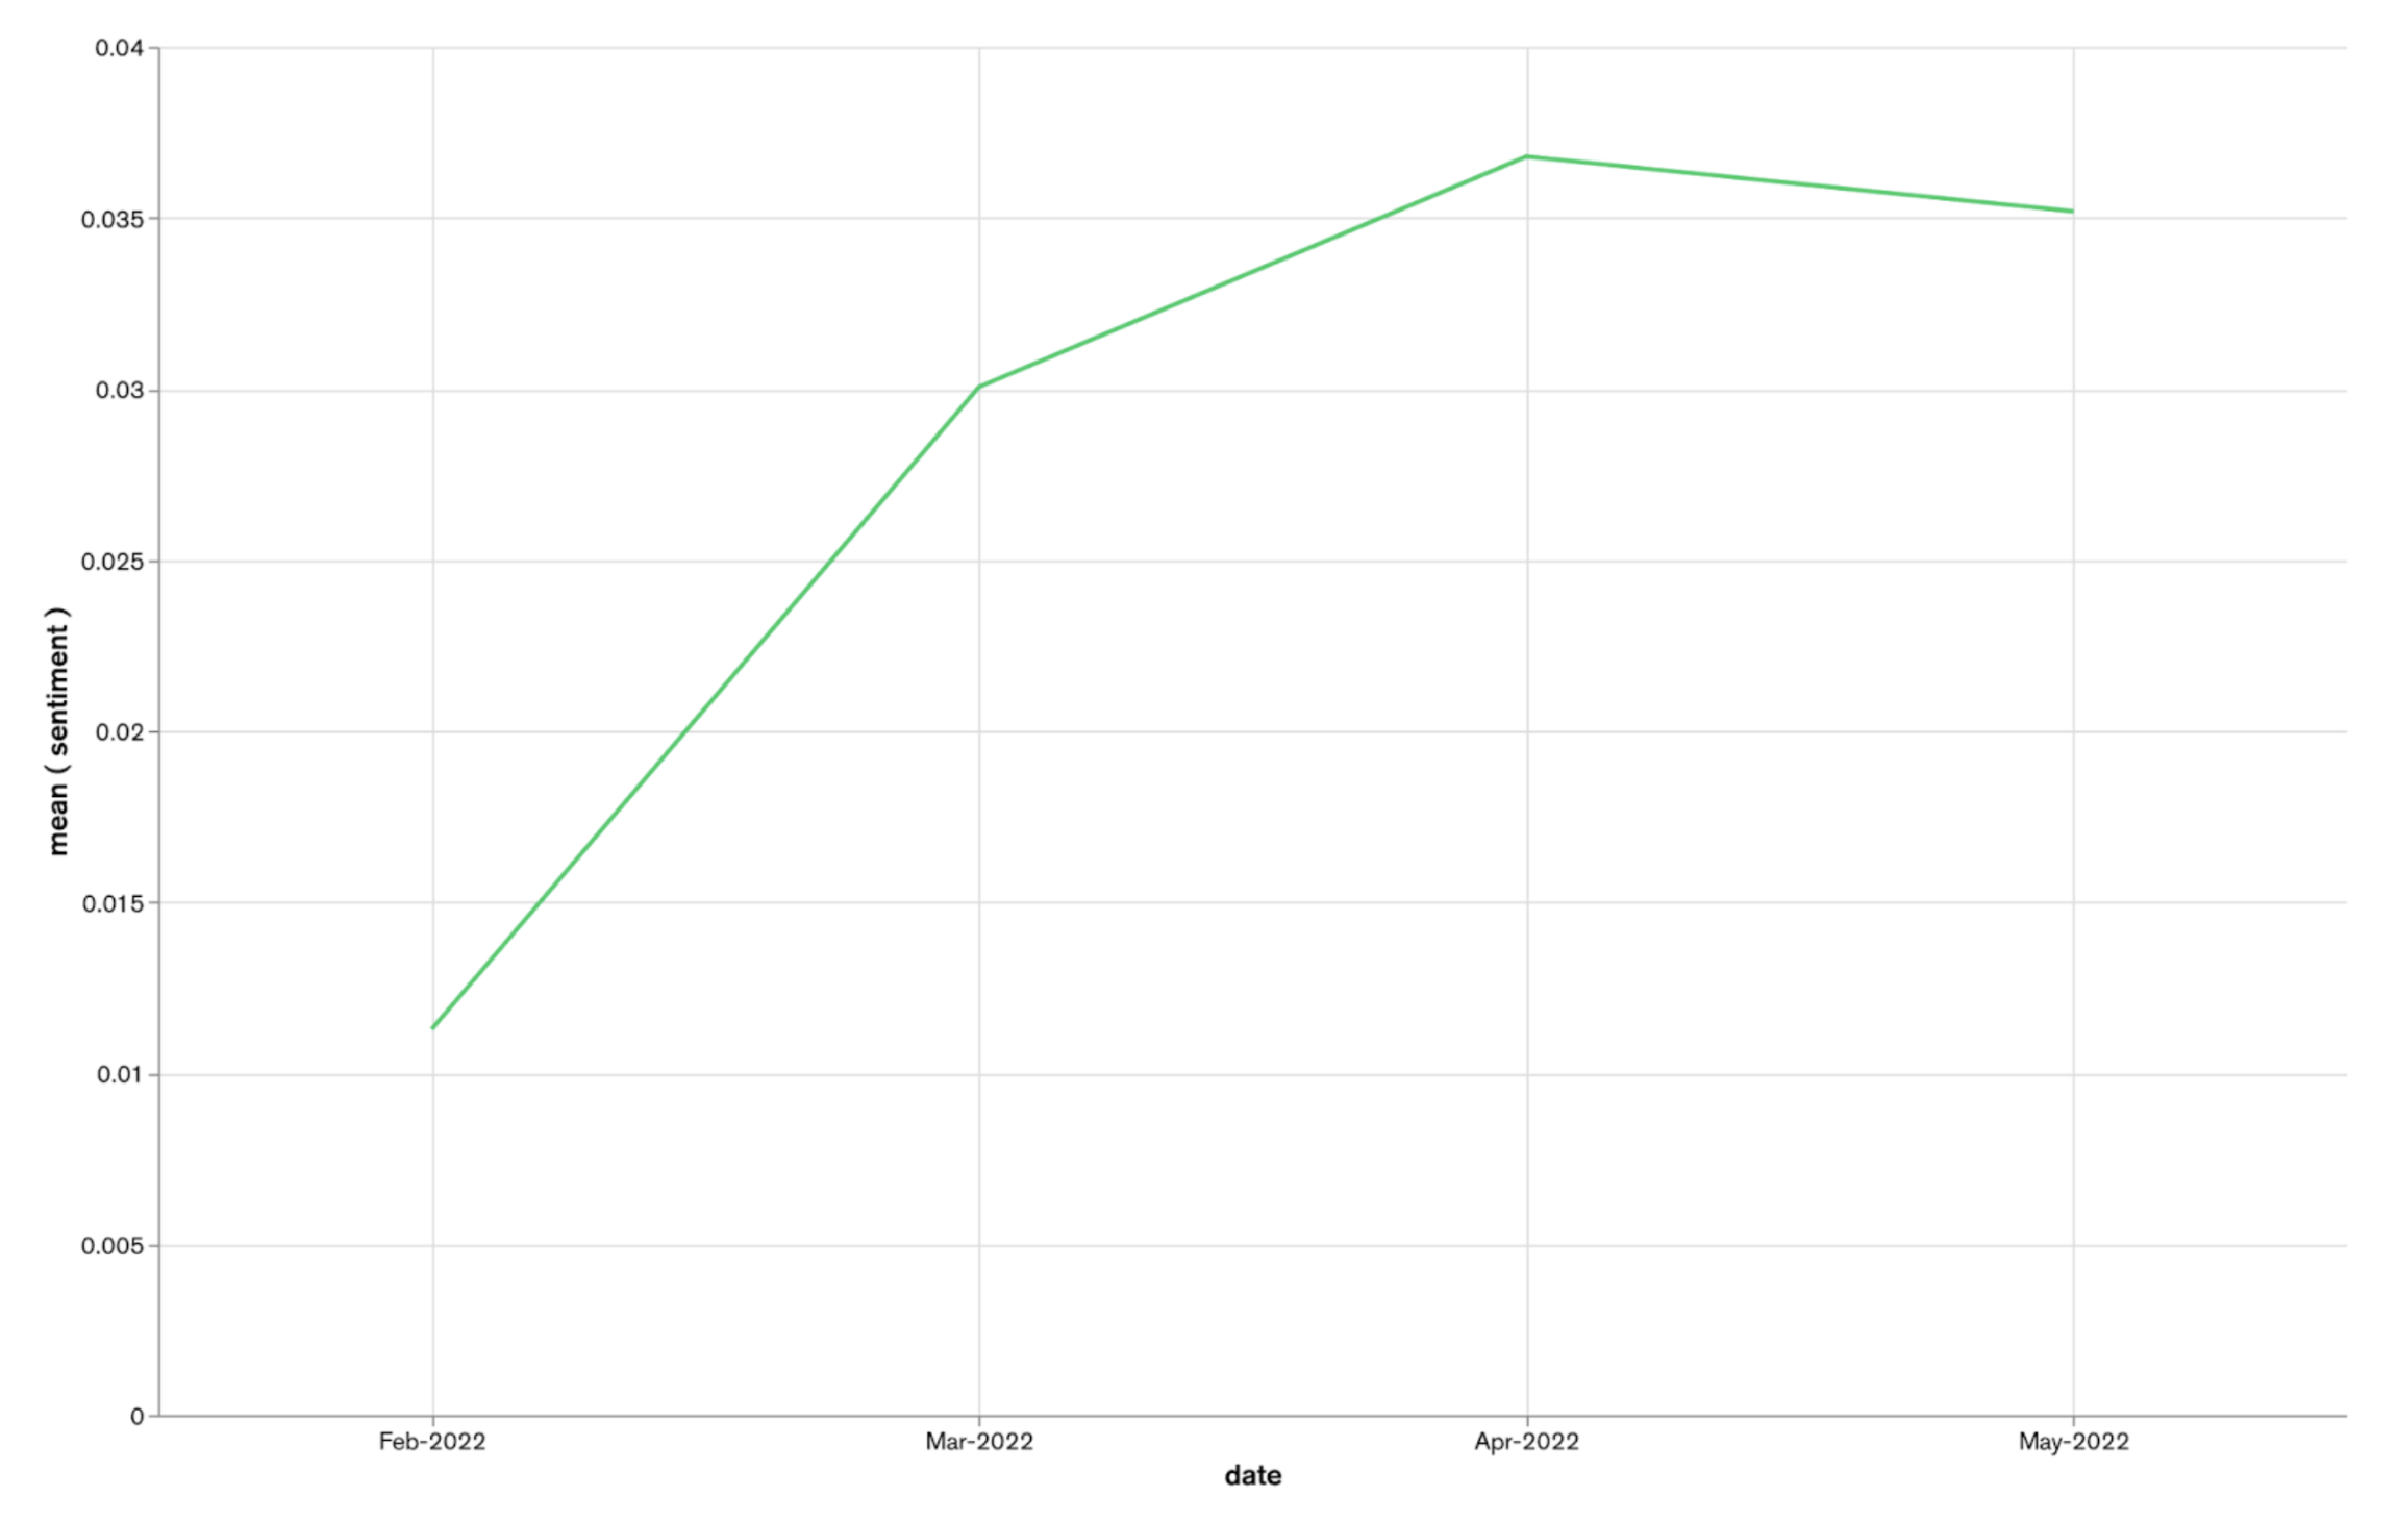
\includegraphics[width=0.8\linewidth]{Thesis/Images/sentiment-by-month.pdf}
	\caption{Average comment sentiment over months}
	\label{fig:sentiment-by-month}
\end{figure}

As can be seen from Figure \ref{fig:sentiment-by-month}, the average comment sentiment is slightly positive but varies over time. The most negative sentiments are observed in February 2022. Potentially, this can be explained by the fact that the escalation of the armed conflict just started in February, and people were confused, stressed and did not know what to expect. Then, the average sentiment goes up in March, and even higher in April. Still, the absolute sentiment values are small and far from being ``definitely positive''. The sentiments are just slightly positive. In May, the sentiment becomes a bit more negative. The fluctuations in the level of sentiment can be explained by the events that occurred in the corresponding months. However, they can also be based on the presence of bots in the online environment.

\section{Development of the web tool}
\subsection{Purpose}
A bot-checking tool developed as a result of this research should present a
web interface available to the public. In this tool, a user should have the possibility to enter the ID or name of a VKontakte user. Then, with the use of the combined model developed in the course of this research, the system should identify whether a user with this ID or name is a bot or not and shows the result to the requesting user. The closest existing analogue is Botometer\footnote{https://botometer.osome.iu.edu/}. However, the difference is that our bot checking tool should work without authentication from the user side and analyse VKontakte accounts instead of Twitter ones.

\subsection{Requirements}
\label{sec:requirements}
Based on the purpose and the core functionality of the web tool, the following requirements were identified:
\begin{enumerate}
    \item Functional:
    \begin{enumerate}
        \item A user must be able to search for VKontakte users from our dataset using either of these values:
        \begin{enumerate}
            \item VKontakte ID;
            \item First name;
            \item Last name.
        \end{enumerate}
        \item A user must be able to see a list of users matching the search query.
        \item A user must be able to check whether a VKontakte user is a bot or a real human, according to the clustering done by our bot detection model.
        \item A user must be able to see the description of the method used to identify bots so that transparency of the system is ensured.
        \item A user must be able to see the web interface author’s contacts so they can get in touch with the author if they have questions or comments.
    \end{enumerate}
    \item Non-functional:
    \begin{enumerate}
        \item The system should be available without registration or authentication.
        \item The system should be publicly available on the Internet.
        \item The system’s design should be accessible.
        \item The system’s design should be responsive to different screen sizes.
        \item The system should be available in three languages:
        \begin{enumerate}
            \item English
            \item Russian
            \item Ukrainian
        \end{enumerate}
    \end{enumerate}
\end{enumerate}

The requirements provided in the list above are essential for the development
of the bot detector web tool. Their implementation is described in the next section.

\subsection{Implementation of the web interface}

The web interface was implemented based on the Flask\footnote{https://flask.palletsprojects.com/en/2.2.x/} framework for Python. Flask allows building web applications in a minimalistic and easy way, providing features both for backend and frontend development with Jinja templates.

In order to ensure the responsiveness and accessibility of the system, an open-source CSS framework Bootstrap\footnote{https://getbootstrap.com/} was used. It provides design templates for typography, forms, buttons and other web UI elements.

\section{Threats to validity}
Sentiment analysis was an essential step in this study. However, the sentiment analysis might have yielded imprecise results for 1,5\% of the dataset (comments written in the Ukrainian language). Since there is no reliable and widely accepted model for sentiment analysis of Ukrainian texts, we analysed the translated version of the comments. During the translation, some parts of the meaning could have been lost.

The absence of ground truth presented a major obstacle and limitation to this research. In general, this is an almost unsolved problem in the whole modern bot detection research field. The most reliable way to obtain the ground truth is to create and inject social bots into social networks. However, this technique did not seem ethical in the context of the ongoing armed conflict. Other tactics of getting the ground truth currently seem to be approximate. Therefore, it is challenging to evaluate the quality of the bot detection models reliably. 

The URL-sharing model, although efficient in detecting specific bots, can only detect coordinated communities that share URLs as part of their influence methods. Other types of bots are not detected by this model.

The web bot detection tool developed during this research only allows retrieving the data about users from the collected database and not about any VKontakte user. Therefore, the applicability of the tool is limited.